% =====================================================================
%  Weave: Distribution-Aware Execution Modeling for Concurrent Go
%  arXiv preprint
%  Compile with: pdflatex weave.tex  (twice, for cross-references)
%  Requires: svproc.cls, aliascnt.sty, remreset.sty  (all at root level)
% =====================================================================
\documentclass{svproc}

\usepackage{url}
\def\UrlFont{\rmfamily}
\usepackage[T1]{fontenc}
\usepackage[utf8]{inputenc}
\usepackage{amsmath,amssymb}
\usepackage{graphicx}
\usepackage{booktabs}
\usepackage{array}
\usepackage{microtype}
\usepackage{xcolor}
\usepackage{listings}
\usepackage{tikz}
\usetikzlibrary{positioning,arrows.meta,fit,calc}

\lstset{basicstyle=\ttfamily\footnotesize,breaklines=true,frame=single,
        columns=fullflexible,keepspaces=true,xleftmargin=0.5em,
        framexleftmargin=0.5em,aboveskip=0.6em,belowskip=0.6em}

% Event-type shorthands
\newcommand{\pblock}{\textsf{GoBlock}}
\newcommand{\punblock}{\textsf{GoUnblock}}
\newcommand{\pstart}{\textsf{GoStart}}
\newcommand{\pcreate}{\textsf{GoCreate}}
\newcommand{\pend}{\textsf{GoEnd}}
\newcommand{\psched}{\textsf{GoSched}}

% Figure colors
\definecolor{cwmblue}{HTML}{2E5E8C}
\definecolor{oursorange}{HTML}{C8552B}
\definecolor{barfill}{HTML}{C8552B}
\definecolor{panelgray}{HTML}{F2F2F2}
\definecolor{panelborder}{HTML}{BBBBBB}
\definecolor{labelone}{HTML}{555555}

\begin{document}
\mainmatter

\title{When the Next Step Is Not One Step:\\
Distribution-Aware Execution Modeling for Concurrent Go Programs}

\titlerunning{Distribution-Aware Execution Modeling for Concurrent Go}

\author{Kaviru Hapuarachchi}
\authorrunning{Hapuarachchi}
\tocauthor{Kaviru Hapuarachchi}
\institute{University of Colombo School of Computing,\\
35 Reid Avenue, Colombo 07, Sri Lanka\\
\email{2022is031@stu.ucsc.cmb.ac.lk}}

\maketitle

% =====================================================================
\begin{abstract}
Training a model to predict the next step in a concurrent program is
harder than it looks: two runs of the same program from the same trace
prefix can produce different next events, both valid, because the
scheduler is nondeterministic. A model trained against a single label
is learning to guess one outcome of a random process. We turn this
around and use the nondeterminism as a training signal. We run each
program many times, aggregate the observed next events into an empirical
distribution, and fine-tune a 7B model to match that distribution with
a KL objective. On 798 held-out predictions drawn from real production
Go bugs (CockroachDB, Kubernetes, gRPC, etcd), fine-tuning on fewer
than a thousand traces reaches 36.2\% accuracy, ahead of Gemini 3.5
Flash used zero-shot (34.8\%) and the same model without fine-tuning
(28.6\%). Distribution training matches cross-entropy on accuracy
(35.8\% vs.\ 36.2\%) while reducing Expected Calibration Error from
0.205 to 0.169. We also derive a formal goroutine-leak signature for a
class of select-blocked goroutines where $P(\punblock)=0$ holds by
scheduler semantics, not by learning. We release the dataset, trained
adapters, and all tooling.
\keywords{concurrent execution modeling; nondeterminism; distribution
estimation; model calibration; Go; goroutine scheduling; concurrency bugs}
\end{abstract}

% =====================================================================
\section{Introduction}
% =====================================================================

A model trained on execution traces learns to predict what a program
does, not just what it looks like. This is the idea behind Code World
Models (CWMs): trained on runtime state snapshots after each statement,
a language model learns the state transition function, which improves
verification, debugging, and code generation~\cite{cwm}. For sequential
Python the approach works well.

But it rests on a quiet assumption: that execution is deterministic.
Given a state and the next statement, there is one next state. For
concurrent code that assumption fails. When goroutines run in parallel
and communicate over channels, the scheduler interleaves them differently
on every run. The same prefix can be followed by a block, a start, or
an unblock, all equally valid. Train a model to predict a single next
event here and you are asking it to memorize one arbitrary outcome of a
random process. It will learn very little.

This is not a minor technicality. Concurrency bugs, deadlocks, data
races, goroutine leaks, have no sequential analogue. They depend on
schedule, evade unit tests, and are hard even for experts to
anticipate~\cite{concur,goker}. If execution-trace models are to be
useful where the bugs are hardest, they must handle the nondeterminism
that defines the setting.

We propose treating the nondeterminism as a signal rather than noise.
Run a concurrent program many times and the distribution of next events
is not random error. It is a measurement of which futures the scheduler
actually permits. We reformulate next-event prediction as distribution
estimation: the target for a prefix is the empirical distribution over
next events observed across repeated runs, and we train a model to match
it (Fig.~\ref{fig:teaser}).

We make the following contributions:

\begin{itemize}
\item We show that a 7B model fine-tuned on fewer than a thousand
  concurrent traces reaches 36.2\% next-event accuracy on held-out
  production bugs from CockroachDB, Kubernetes, gRPC, and etcd,
  beating Gemini 3.5 Flash zero-shot (34.8\%) and the same
  model without fine-tuning (28.6\%).
\item We show that training with a KL objective against empirical
  distributions matches cross-entropy on accuracy (35.8\% vs.\ 36.2\%)
  while improving calibration: Expected Calibration Error drops from
  0.205 to 0.169 and model entropy correlates with program
  nondeterminism.
\item We derive a formal leak signature for select-blocked goroutines,
  showing that $P(\punblock)=0$ at every trace depth follows from Go
  scheduler semantics, not from learning.
\item We report where the approach falls short: accuracy plateaus near
  35--36\% regardless of model or objective, rare event types are never
  learned, and multi-step predictions lose scheduler coherence after
  roughly one step.
\end{itemize}

We are not claiming a deployable bug detector or a production-ready
execution simulator. The contribution is a formulation, a dataset, and
a set of baselines that show nondeterminism-aware training works and
make clear what would need to change for it to work better.

% =====================================================================
\begin{figure}[t]
\centering
\resizebox{\linewidth}{!}{%
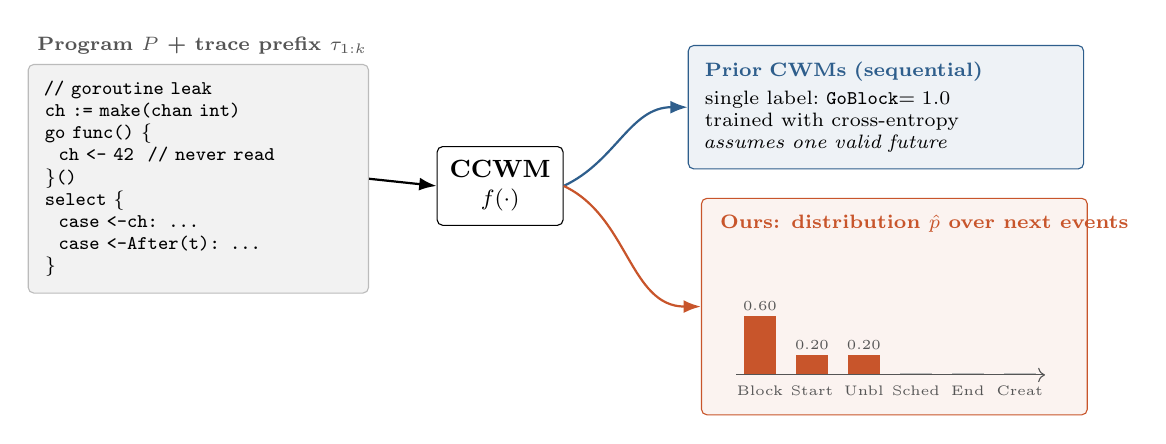
\begin{tikzpicture}[font=\sffamily]

\node[anchor=north west,align=left,font=\ttfamily\scriptsize,
      fill=panelgray,draw=panelborder,rounded corners=2pt,
      inner sep=6pt,text width=3.9cm] (prog) at (0,0)
{// goroutine leak\\
ch := make(chan int)\\
go func() \{\\
\ \ ch <- 42 \ // never read\\
\}()\\
select \{\\
\ \ case <-ch: ...\\
\ \ case <-After(t): ...\\
\}};
\node[anchor=south west,font=\bfseries\scriptsize,labelone]
      at (prog.north west) {Program $P$ + trace prefix $\tau_{1:k}$};

\node[draw,fill=white,rounded corners=2pt,minimum height=1.0cm,
      minimum width=1.6cm,align=center,font=\small\bfseries]
      (model) at (6.0,-1.55) {CCWM\\[-1pt]\footnotesize $f(\cdot)$};
\draw[-{Latex[length=2.2mm]},thick] (prog.east) -- (model.west);

\node[draw=cwmblue,fill=cwmblue!8,rounded corners=2pt,
      inner sep=6pt,align=left,font=\scriptsize,text width=4.6cm]
      (cwm) at (10.9,-0.55)
{\textbf{\color{cwmblue}Prior CWMs (sequential)}\\[2pt]
single label:\ \texttt{GoBlock}$=1.0$\\
trained with cross-entropy\\
\emph{assumes one valid future}};

\node[draw=oursorange,fill=oursorange!7,rounded corners=2pt,
      minimum width=4.9cm,minimum height=2.75cm,anchor=north west]
      (ourspanel) at (8.55,-1.7) {};
\node[anchor=north west,font=\scriptsize\bfseries,oursorange,align=left]
      at ($(ourspanel.north west)+(0.12,-0.1)$)
      {Ours: distribution $\hat p$ over next events};

\begin{scope}[shift={($(ourspanel.north west)+(0.55,-2.25)$)}]
  \def\gap{0.66}\def\bw{0.40}\def\h{1.25}
  \foreach \i/\p/\lab in {0/0.60/Block,1/0.20/Start,2/0.20/Unbl,3/0.00/Sched,4/0.00/End,5/0.00/Creat}{
    \pgfmathsetmacro\bh{\p*\h}
    \ifdim\bh pt>0.01pt
      \fill[barfill] ({\i*\gap},0) rectangle ({\i*\gap+\bw},{\bh});
      \node[font=\tiny,labelone] at ({\i*\gap+\bw/2},{\bh+0.13}) {\p};
    \else
      \draw[panelborder] ({\i*\gap},0) rectangle ({\i*\gap+\bw},0.02);
    \fi
    \node[font=\tiny,labelone,anchor=north] at ({\i*\gap+\bw/2},-0.02) {\lab};
  }
  \draw[->,labelone] (-0.1,0) -- ({5*\gap+\bw+0.12},0);
\end{scope}

\draw[-{Latex[length=2.2mm]},thick,cwmblue] (model.east) to[out=25,in=180] (cwm.west);
\draw[-{Latex[length=2.2mm]},thick,oursorange] (model.east) to[out=-25,in=180]
      ($(ourspanel.west)+(0,0.0)$);

\end{tikzpicture}}%
\caption{Concurrent execution has many valid next steps, not one. Prior
Code World Models (blue) predict a single next event and train against
it with cross-entropy, which works for sequential code but is
ill-defined when the same prefix can legitimately produce several
different events. We predict a full distribution over next events
(orange), with targets derived from repeated runs of the same program.
The right panel shows an example distribution for a goroutine-leak
program: \pblock\ dominates and $P(\punblock)=0$, a signature that
follows from the scheduler, not from learning.}
\label{fig:teaser}
\end{figure}
% =====================================================================

% =====================================================================
\section{Background and Related Work}\label{sec:related}
% =====================================================================

\textbf{Code world models and execution traces.}
A world model learns an environment's transition function: state and
action in, next state out~\cite{cwm}. CWMs apply this to program
execution, training on action-state pairs from interpreter traces so
the model predicts the next action and resulting state from a partial
trace~\cite{cwm}. Meta's 32B CWM, trained on Python traces and agentic
trajectories, showed that this grounding improves coding and
reasoning~\cite{cwm}. A follow-up study of CWM failure modes found that
errors concentrate in two regimes: token-budget exhaustion on long
traces and string-valued state confused by subword
tokenization~\cite{debugcwm}. Both studies assume deterministic,
sequential execution.

\textbf{Concurrency and LLMs.}
Concurrent code introduces nondeterministic scheduling and bug classes,
races, deadlocks, starvation, that have no sequential equivalent.
Unit-test evaluation cannot systematically explore thread
schedules~\cite{concur}. The CONCUR benchmark targets concurrent code
generation, judged by model checking~\cite{concur}. Our problem is
different: modeling the execution of concurrent programs as a learned
transition function, using scheduling nondeterminism as a distributional
target. The GoKer/GoBench corpus of real Go concurrency
bugs~\cite{goker} provides our held-out test programs.

\textbf{Distribution matching and calibration.}
Training against a target distribution rather than a point label is an
established technique: soft-target objectives improve language-model
calibration, often using an empirical distribution from a few hundred
samples as the target~\cite{diffuse,probcalib}. Our contribution is not
distribution matching itself but its source. The nondeterminism of
concurrent execution, observed through repeated runs, gives a
principled empirical target over next events. We are not aware of prior
work deriving distributional training targets from concurrent execution
traces.

Table~\ref{tab:position} positions our work against the two closest
lines of prior research.

\begin{table}[t]
\centering
\caption{Comparison against prior execution-trace modeling and the
closest concurrency benchmark across dimensions relevant to this
problem. This work is the first to combine execution-trace modeling
with concurrent programs and nondeterministic distributional targets.}
\label{tab:position}
\small
\begin{tabular}{lccc}
\toprule
 & \textbf{Sequential CWM} & \textbf{CONCUR} & \textbf{This work}\\
 & \cite{cwm} & \cite{concur} & \\
\midrule
Concurrent programs        & no  & yes & yes\\
Models execution (vs.\ gen.) & yes & no  & yes\\
Nondeterministic targets   & no  & n/a & yes\\
Real-world bug test set    & no  & no  & yes (GoKer)\\
Calibration evaluated      & no  & no  & yes\\
\bottomrule
\end{tabular}
\end{table}

% =====================================================================
\section{Problem Formulation}\label{sec:problem}
% =====================================================================

We consider Go programs that spawn multiple goroutines. The runtime
tracer emits scheduler events and we work with six event types covering
goroutine lifecycle and synchronization:
\[
\mathcal{E}=\{\pblock,\ \pcreate,\ \pend,\ \psched,\ \pstart,\ \punblock\}.
\]
A trace is a sequence of snapshots $\tau=(s_1,\dots,s_n)$, each
recording the triggering event type, the goroutine id, and per-goroutine
status (running / runnable / blocked / dead). Given a prefix $\tau_{1:k}$
and program source $P$, the task is to predict the event type of $s_{k+1}$.

\textbf{From label to distribution.}
Standard CWM training takes the next event as one label and minimizes
cross-entropy. Because execution is nondeterministic, repeated runs of
$P$ from comparable prefixes produce different valid next events. For a
group $g$ of runs sharing a program and prefix depth, let $c_g(e)$ count
next events of type $e$. The empirical distribution and its Dirichlet
posterior (Jeffreys prior $\alpha{=}0.5$) are
\begin{equation}
\hat{p}_g(e)=\frac{c_g(e)}{\sum_{e'}c_g(e')},\qquad
\tilde{\alpha}_g(e)=\alpha + c_g(e).
\end{equation}
The learning target is $\hat p_g$, not a single label. We approximate
``same prefix'' by matching split depths (25/50/75\% of the trace). Because
interleavings differ across runs, grouped prefixes are structurally
comparable but not byte-identical. We revisit this approximation in
Section~\ref{sec:threats}.

% =====================================================================
\section{Dataset and Evaluation Setup}\label{sec:data}
% =====================================================================

\textbf{Programs.}
We assembled 130 concurrent Go programs in three groups
(Table~\ref{tab:corpus}). Hand-crafted programs cover channel, mutex,
select, pipeline, waitgroup, and fan-in/out patterns, with intentional
deadlocks, races, and leaks. Generated programs are synthesized with
randomized parameters and optional injected bugs, each verified to
compile. Real-world programs are reduced concurrency-bug kernels from
the GoKer/GoBench corpus~\cite{goker}, drawn from production systems
including CockroachDB, Kubernetes, gRPC, etcd, Istio, and Moby. Each
program carries metadata describing outcome, pattern, goroutine count,
and expected nondeterminism.

\begin{table}[t]
\centering
\caption{Program corpus. All 66 real-world GoKer programs are held out
from training, so accuracy on those programs measures out-of-distribution
generalization to code the model never saw during fine-tuning.}
\label{tab:corpus}
\small
\begin{tabular}{lcl}
\toprule
\textbf{Group} & \textbf{Count} & \textbf{Source}\\
\midrule
Hand-crafted & 26 & All patterns; intentional bugs\\
Generated    & 38 & Parameterized synthesis with injected bugs\\
Real-world   & 66 & GoKer/GoBench kernels (held out for test)\\
\midrule
\textbf{Total} & \textbf{130} & \\
\bottomrule
\end{tabular}
\end{table}

\textbf{Traces.}
Each program is compiled with the race detector and run five times under
the runtime tracer. Differing interleavings across runs are the
variability we exploit. From each run we form examples at 25/50/75\%
prefix depth. Deadlocking programs emit a no-next-event marker and are
excluded from distribution aggregation. The tracer exposes scheduler
events but not channel buffers, mutex holders, or local variables, so
the model must reason from scheduling behavior and program structure.

\textbf{Splits.}
We hold out all 66 real-world programs for evaluation and train only on
hand-crafted and generated programs. This yields 945 training examples
and 798 held-out next-event predictions, plus 75 aggregated
empirical-distribution groups.

% =====================================================================
\section{Method}\label{sec:method}
% =====================================================================

\textbf{Format.}
Each example renders the program source, the partial trace as JSON, and
the current goroutine states, then asks for the next event. The point
target is a JSON object \texttt{\{"event\_type":..., "goroutine\_id":...\}};
the distribution target is the six-way vector $\hat p_g$. Prompts are
left-truncated at the source so the target is never cut off.

\textbf{Cross-entropy baseline.}
We fine-tune Qwen2.5-Coder (1.5B and 7B) with cross-entropy over
response tokens using 4-bit QLoRA (rank 16, $\alpha{=}32$, gradient
checkpointing). To approximate the empirical distribution under a point
loss, examples are duplicated in proportion to observed next-event
frequency.

\textbf{KL distribution loss.}
The distribution objective adds a KL term at the token position that
discriminates between event types. With logits $z$ restricted to the
six event-type tokens, $q=\mathrm{softmax}(z)$, and empirical target
$\hat p_g$,
\begin{equation}
\mathcal{L}=\mathcal{L}_{\mathrm{CE}}+\lambda\,\mathrm{KL}(\hat p_g \,\|\, q),
\end{equation}
with $\lambda{=}0$ recovering the CE ablation. Because all six event
types share the leading subword ``Go,'' we place the KL term at the
second, discriminating token. The 7B QLoRA configuration is identical
to the CE baseline so that any difference is attributable to the
objective alone.

\textbf{Multi-step coherence probe.}
To measure how far single-step prediction extends before it breaks, we
feed the model's own predictions back as input: from a real prefix,
predict the next event, append it, and repeat for up to 15 steps. A
symbolic scheduler finite-state machine checks each predicted transition
against Go invariants (for example, a blocked goroutine cannot be
started). We report survival steps, meaning valid transitions before
the first violation, along with the per-step event distribution and
entropy. We use this as a diagnostic tool in Section~\ref{sec:analysis}
to locate the boundary between what the model can and cannot do.

% =====================================================================
\section{Results}\label{sec:results}
% =====================================================================

\begin{table}[t]
\centering
\caption{Next-event accuracy on the held-out real-world GoKer set.
Fine-tuning on concurrent traces from hand-crafted programs generalizes
to real production bugs, outperforming both the zero-shot baseline and
Gemini 3.5 Flash. Distribution training with KL loss achieves
comparable accuracy to cross-entropy while improving calibration
(Section~\ref{sec:analysis}).}
\label{tab:ood}
\small
\begin{tabular}{p{6.8cm}c}
\toprule
\textbf{Model} & \textbf{Accuracy}\\
\midrule
Qwen2.5-Coder-7B, zero-shot             & 28.6\%\\
Gemini 3.5 Flash, with thinking         & 34.8\%\\
Gemini 3.5 Flash, no thinking           & 35.2\%\\
Qwen2.5-Coder-7B, fine-tuned KL (ours) & 35.8\%\\
Qwen2.5-Coder-7B, fine-tuned CE (ours) & \textbf{36.2\%}\\
\bottomrule
\end{tabular}
\end{table}

\begin{table}[t]
\centering
\caption{In-distribution accuracy on hand-crafted programs, included
for context. These numbers are not directly comparable to
Table~\ref{tab:ood} because the model used here is an earlier Gemini
generation evaluated with a different prompt format.}
\label{tab:indist}
\small
\begin{tabular}{p{6.8cm}c}
\toprule
\textbf{Model} & \textbf{Accuracy}\\
\midrule
Qwen2.5-Coder-1.5B, zero-shot             & 29.8\%\\
Gemini (earlier gen., different prompt)   & 56.0\%\\
Qwen2.5-Coder-1.5B, fine-tuned CE (ours) & \textbf{40.2\%}\\
\bottomrule
\end{tabular}
\end{table}

\textbf{Fine-tuning generalizes out-of-distribution.}
Table~\ref{tab:ood} shows the main result. Trained on 945 hand-crafted
and generated traces, a 7B model reaches 36.2\% on real-world GoKer bugs
it never saw during training. This beats the same model zero-shot
(28.6\%) and Gemini 3.5 Flash used zero-shot (34.8--35.2\%).
Small-scale concurrent-trace supervision transfers to structurally
different real code.

\textbf{Distribution training matches accuracy.}
KL training reaches 35.8\%, which is not meaningfully different from
CE's 36.2\%. We view this as the expected outcome: distribution training
should not sacrifice accuracy, and the benefit appears in calibration
rather than top-1 prediction (Section~\ref{sec:analysis}).

\textbf{An accuracy ceiling near 35--36\%.}
Three approaches, CE fine-tuning, KL fine-tuning, and a strong zero-shot
model, all land within one percentage point of each other. That
clustering is itself informative: predicting the next scheduler event of
a real concurrency bug from traces alone is hard, and neither scale nor
objective moves the ceiling. Section~\ref{sec:analysis} traces this to
rare events and distribution shift.

\textbf{Reasoning does not help.}
Enabling thinking in Gemini 3.5 Flash slightly lowers accuracy
(34.8\% vs.\ 35.2\%). The relevant signal here is structural, not
multi-step deductive.

% =====================================================================
\section{Analysis: Where the Ceiling Comes From}\label{sec:analysis}
% =====================================================================

\textbf{Per-event accuracy.}
Table~\ref{tab:perevent} breaks accuracy down by event type. The model
learns common lifecycle events, \pstart\ at 47\%, \pcreate\ at 44\%,
\pblock\ at 36\%, but never predicts \pend\ or \psched\ (both 0\%) and
rarely gets \punblock\ right (8\%).

\begin{table}[t]
\centering
\caption{Per-event accuracy of the KL model on GoKer, alongside train
and test frequency. Two events with near-zero training frequency,
\pend\ and \psched, are never predicted correctly. Meanwhile \pcreate\
achieves 44\% accuracy from only 1.5\% of training examples, suggesting
the model reasons from program structure rather than label frequency.}
\label{tab:perevent}
\small
\begin{tabular}{lccc}
\toprule
\textbf{Event} & \textbf{Train freq.} & \textbf{Test freq.} & \textbf{Accuracy}\\
\midrule
\pstart   & 42\%  & 35\% & 47\%\\
\pblock   & 37\%  & 26\% & 36\%\\
\punblock & 17\%  & 6\%  & 8\%\\
\pcreate  & 1.5\% & 21\% & 44\%\\
\pend     & 2\%   & 4\%  & 0\%\\
\psched   & 0.4\% & 7\%  & 0\%\\
\bottomrule
\end{tabular}
\end{table}

Two effects compound to produce the ceiling. First, class imbalance:
\pend\ (2\%) and \psched\ (0.4\%) are so rare in training that the model
never emits them, and KL does not fix this because the empirical targets
are themselves skewed toward common events. Second, distribution shift:
real GoKer programs exercise \pcreate\ (21\% of test) and \psched\ (7\%)
far more than the hand-crafted training set does. The \pcreate\ result
is worth noting: 44\% accuracy from only 1.5\% of training examples
means the model is picking up structural cues from the program text, not
just frequency patterns.

\textbf{Calibration and uncertainty.}
Beyond top-1 accuracy, distribution framing improves how well predicted
probabilities track reality. In a prompting study over the aggregated
groups, predicting a distribution with a reasoning budget lowers Expected
Calibration Error from 0.205 (point-prediction baseline) to 0.169, and
model entropy correlates with program nondeterminism (Spearman
$\rho=0.412$, $p=0.007$). In the multi-step probe, the KL model assigns
higher entropy to harder programs: 0.945 bits on leak programs vs.\
0.773 on race programs. This is uncertainty the cross-entropy model
cannot express by design.

\textbf{The single-step boundary.}
Table~\ref{tab:rollout} summarizes the 15-step coherence probe on 54
GoKer programs. The first predicted step reflects real execution
semantics: on leak programs, predictions are \pblock-dominated with
$P(\punblock)$ near zero, matching the signature described in
Section~\ref{sec:signature}. However, mean survival is roughly one step
before the model produces a scheduler-invalid transition. This was
expected: the model was trained only on single steps, so using its
predictions autoregressively exposes the boundary quickly. The probe is
useful because it locates that boundary precisely rather than leaving it
as an open question.

\begin{table}[t]
\centering
\caption{Multi-step coherence probe on GoKer (15 steps, 3 samples per
program). The first predicted step reflects the leak signature, but
mean survival drops to roughly one step before the model produces
invalid transitions, confirming that single-step training does not
transfer to multi-step simulation.}
\label{tab:rollout}
\small
\begin{tabular}{lcccc}
\toprule
\textbf{Outcome} & \textbf{$n$} & \textbf{Dominant event} & \textbf{Survival} & \textbf{Entropy}\\
\midrule
Leak & 37 & \pblock\ (50\%) & 1.11 steps & 0.945 bits\\
Race & 17 & \pblock\ (65\%) & 0.67 steps & 0.773 bits\\
\bottomrule
\end{tabular}
\end{table}

% =====================================================================
\section{The Select-Block Leak Signature}\label{sec:signature}
% =====================================================================

One distributional pattern in our data has a formal explanation rather
than a statistical one. In a subclass of goroutine leaks, we consistently
observe $P(\punblock)=0$ at every trace depth across all five runs of
those programs.

Consider a goroutine $G$ that enters a \texttt{select} statement at
time $t$, where none of the case conditions can ever be satisfied by the
remaining execution. We call this a \emph{select-block leak}. For such
$G$, a \punblock\ event is impossible for all $t' > t$, and so
$P(\punblock)=0$ in the empirical next-event distribution for any split
taken after $G$'s first \pblock.

The reason is straightforward. In Go, \punblock\ fires only when another
goroutine sends to or closes a channel that $G$ is waiting on, or
releases a mutex that $G$ is waiting to acquire. If no reachable
goroutine in the remaining execution can do either, then \punblock\
never fires. This is a consequence of the scheduler's semantics, not
something the model learns. It holds regardless of how many
\texttt{select} cases $G$ has; we verified this for both two-case and
four-case selects.

The signature is mechanism-specific and we are careful not to overstate
it. Only leaks where the goroutine reaches a permanently blocked select
\emph{before} any \punblock\ event appears in the trace show the
all-zero pattern. Leaks that do legitimate work first, for example
receiving items from a channel before blocking, show $P(\punblock)>0$
at early split depths. We tried using this signal as an unsupervised
anomaly detector and found it separates buggy from clean programs only
weakly at our scale (Cohen's $d=0.29$, not significant at $n{=}9$).
We present it as a precise characterization of one leak class, not as
a general-purpose detector.

% =====================================================================
\section{Threats to Validity}\label{sec:threats}
% =====================================================================

Our grouping of runs by split depth is an approximation. We treat runs
at the same depth as sharing a prefix family, but because interleavings
differ, the actual prefixes are structurally comparable rather than
identical. This can blur the empirical distribution targets, particularly
for programs with high nondeterminism where many interleavings are
equally likely.

The runtime tracer does not expose channel buffer occupancy, mutex
ownership, or local variable values. The model reasons from a partial
view of program state, which bounds achievable accuracy and explains
some of the confusion in event types like \punblock\ that depend on
synchronization state the model cannot see.

Several of our secondary analyses rest on small samples. The calibration
correlation ($\rho=0.412$, $p=0.007$) is statistically significant, but
the anomaly detection result ($n{=}9$, Cohen's $d=0.29$) is not. We
report effect sizes throughout rather than drawing conclusions from
isolated $p$-values.

The in-distribution Gemini result in Table~\ref{tab:indist} used
an earlier model generation and a different prompt format. We include
it to show the relative improvement from fine-tuning, but we do not
compare it numerically to the out-of-distribution results in
Table~\ref{tab:ood}.

% =====================================================================
\section{Conclusion}\label{sec:conclusion}
% =====================================================================

We reformulated next-event prediction for concurrent programs as
distribution estimation over empirical nondeterministic targets. A 7B
model fine-tuned on fewer than a thousand Go traces generalizes to real
production concurrency bugs better than a strong zero-shot large model,
and distribution training with a KL objective matches cross-entropy
accuracy while improving calibration. The 35--36\% accuracy ceiling
traces to rare-event failure and train-test distribution shift, and
multi-step predictions lose coherence after roughly one step because the
model was never trained on trajectories.

Three directions follow directly from these findings. Training on
trajectories rather than individual steps is the most direct path to
extending multi-step coherence. Encoding channel and mutex state in the
trace representation would let the model reason about synchronization,
not just goroutine lifecycle events. Rebalancing the training set toward
the event mix of real Go code would address the class-imbalance ceiling
that currently prevents the model from learning rare but important event
types. We release the dataset, the cross-entropy and KL adapters, and
all tooling to support this line of work.

% =====================================================================
\section*{Appendix: Artifacts and Compute}
% =====================================================================

All artifacts are publicly released. Code, tooling, and scripts are
available at~\cite{weave-repo}. The benchmark dataset is
released as~\cite{weave-bench}. The cross-entropy and KL fine-tuned
7B adapters are released as~\cite{weave-ce} and~\cite{weave-kl}
respectively; both are 4-bit QLoRA adapters runnable on a single
20\,GB GPU.

Total compute cost was \$12 for fine-tuning on a RunPod RTX~4000~Ada
and \$60 for Gemini API inference across all zero-shot evaluations.

% =====================================================================
\begin{thebibliography}{9}
% =====================================================================

\bibitem{cwm}
FAIR CodeGen Team:
CWM: An Open-Weights LLM for Research on Code Generation with World Models.
arXiv:2510.02387 (2025)

\bibitem{debugcwm}
Rahmani, B.:
Debugging Code World Models.
arXiv:2602.07672 (2026)

\bibitem{concur}
Huang, J., Mahmud, T., P\u{a}s\u{a}reanu, C., Yang, G.:
CONCUR: Benchmarking LLMs for Concurrent Code Generation.
arXiv:2603.03683 (2026)

\bibitem{goker}
Tu, T., Liu, X., Song, L., Zhang, Y.:
Understanding Real-World Concurrency Bugs in Go.
In: ASPLOS (2019)

\bibitem{diffuse}
Zhang, Y., Schwarzschild, A., Carlini, N., Kolter, Z., Ippolito, D.:
Forcing Diffuse Distributions out of Language Models.
arXiv:2404.10859 (2024)

\bibitem{probcalib}
Baldelli, D., Kuriakose, S., Hashemzadeh, M., Zouaq, A., Chandar, S.:
Probabilistic Calibration Is a Trainable Capability in Language Models.
arXiv:2605.11845 (2026)

\bibitem{weave-repo}
Hapuarachchi, K.:
Weave: Concurrent Code World Models -- Code, Tooling, and Evaluation Scripts.
\url{https://github.com/kaviru2/weave} (2026)

\bibitem{weave-bench}
Hapuarachchi, K.:
weave-bench: Concurrent Go Execution Trace Benchmark Dataset.
HuggingFace Datasets.
\url{https://huggingface.co/datasets/kavirubc/weave-bench} (2026)

\bibitem{weave-ce}
Hapuarachchi, K.:
weave-ccwm-qwen2.5-coder-7b-lora: Cross-Entropy Fine-Tuned Adapter.
HuggingFace.
\url{https://huggingface.co/kavirubc/weave-ccwm-qwen2.5-coder-7b-lora} (2026)

\bibitem{weave-kl}
Hapuarachchi, K.:
weave-ccwm-qwen2.5-coder-7b-kl-lora: KL Distribution Fine-Tuned Adapter.
HuggingFace.
\url{https://huggingface.co/kavirubc/weave-ccwm-qwen2.5-coder-7b-kl-lora} (2026)

\end{thebibliography}

\end{document}
